\documentclass[letterpaper,10pt,conference]{ieeeconf}
\overrideIEEEmargins
\usepackage{amsmath,amsfonts,amssymb}
\usepackage{algorithmic}
\usepackage{algorithm}
\usepackage{array}
\usepackage{tabularx}
\usepackage{booktabs}
\usepackage{threeparttable}
\newcolumntype{Y}{>{\centering\arraybackslash}X}
\newcolumntype{L}{>{\raggedright\arraybackslash}X}
\usepackage{textcomp}
\usepackage{stfloats}
\usepackage{url}
\usepackage{verbatim}
\usepackage{graphicx}
\usepackage{cite}

\usepackage{bm}
\usepackage{pifont}
\newtheorem{lemma}{Lemma}
\newtheorem{proposition}{Proposition}
\newtheorem{theorem}{Theorem}
\newtheorem{corollary}{Corollary}
\newtheorem{remark}{Remark}
\usepackage{xcolor}
\newcommand{\rev}[1]{\textcolor{blue}{#1}}
\newcommand{\nd}[1]{\textcolor{red}{#1}}
\newcommand{\todo}[1]{\textcolor{red}{\textbf{[TODO: #1]}}}
\newcommand{\draftnote}[1]{\par\noindent\textcolor{red}{\textbf{$\blacktriangleright$ DRAFT: #1}}\par\medskip}
\newcommand{\figph}[2]{\fcolorbox{red}{gray!8}{\parbox[c][#1][c]{0.96\linewidth}{\centering
\color{red!65!black}\small\textbf{[figure placeholder]}\\[3pt] #2}}}
\graphicspath{{figs/}}
\hyphenation{op-tical net-works semi-conduc-tor IEEE-Xplore Koop-man}

% ---- method-name macros (freeze notation here) ----
\newcommand{\mbdtrue}{\textsc{MBD-true}}
\newcommand{\dkmbd}{\textsc{DK-MBD}}
\newcommand{\dksplit}{\textsc{DK-MBD-split}}
\newcommand{\bkmbd}{\textsc{BK-MBD}}
\newcommand{\dklarge}{\textsc{DK-MBD-large}}
\newcommand{\mlpmbd}{\textsc{MLP-MBD}}

% \usepackage[hidelinks]{hyperref}
\usepackage{hyperref}
\usepackage{subcaption}
% (a)/(b) subfigure labels in Times New Roman (ptm = Times); caption text unchanged
\DeclareCaptionFont{timesnr}{\fontfamily{ptm}\selectfont}
\captionsetup[subfigure]{labelfont=timesnr}

\begin{document}

\title{Koopman-Accelerated Model-Based Diffusion for Real-Time Robot Control}

% Author intentionally omitted for blind submission.
% \author{Author Name(s)\thanks{Affiliation / funding.}}

\maketitle

\begin{abstract}

\end{abstract}

\noindent\textbf{Keywords---}Koopman operator, sampling-based control,
model-based diffusion, data-driven control, model learning for control.

%==============================================================
\section{Introduction}\label{sec:intro}
%==============================================================

Sampling-based predictive control is widely used on robotic systems with nonlinear dynamics.
MPPI~\cite{kappen2005, theodorou2010, williams2017mppi, williams2016aggressive} and Model-Based Diffusion (MBD)~\cite{pan2024model} score a population of candidate control sequences by forward rollout and update the nominal sequence by a cost-weighted average.
MBD reads that update as one step of reverse diffusion.
The weighted mean estimates the score of a Gaussian-smoothed target~\cite{song2019generative, song2020score}, and a decreasing noise schedule moves the search from coarse to fine.
Neither the cost nor the feasible set has to be differentiable or convex.

The rollout model keeps MBD out of the control loop.
One control step evaluates the rollout once per candidate at every annealing stage, and receding-horizon control draws a new population after each executed action.
MBD is posed as an offline trajectory optimizer, and its use under receding horizon is left open~\cite{pan2024model}.
Rolling a population through a simulation of the plant is the dominant cost of a control step, and Xue et al.~\cite{xue2025full} later carried that cost on a vectorized physics engine, running annealed sampling at the control rate and leaving the rollout model unchanged.
Reaching the control rate on a CPU requires a rollout model cheaper than a simulation of the plant.

Replacing the simulator raises a question the simulator never posed.
Where must the surrogate be accurate?
The sampling weights read only differences of cost within a population, and the candidates differ in the control sequence alone.
An error the surrogate commits independently of the input leaves the weights unchanged.
An error in the path by which the input reaches the tracked output reorders the candidates.

A Koopman lift supplies such a surrogate.
Lifting the state through hand-designed~\cite{williams2015edmd, proctor2016dmdc} or learned~\cite{lusch2018deep} observables turns a nonlinear rollout into repeated matrix--vector products whose cost the lifted dimension sets.
Hao et al.~\cite{mppidk2026} placed a learned linear Koopman model inside an MPPI loop for this reason.
A linear lift receives the input through a constant matrix, so a command moves the tracked output in the same way at every configuration.
On a velocity-commanded platform the command is issued in a joint or body frame and the tracked output lives in the world frame.
The map between the two frames turns with the configuration and ranges over its full extent across the postures a task visits.
A constant matrix matches it at one posture.

Bilinear Koopman realizations multiply the lifted state by the input and restore a configuration-dependent input map~\cite{iacob2024}.
Lifted predictive control nonetheless builds mostly on the linear form, for which the online problem is a quadratic program~\cite{korda2018mpc}.
Bruder et al.~\cite{bruder2021bilinear} identified a bilinear model from data, but the bilinear term breaks convexity, so they froze the lifted state along a nominal trajectory.
That remedy removes the state dependence the bilinear form was adopted for.
The optimizer, not the model, has kept the bilinear class out of this role.
A sampling planner scores whole candidate sequences by the cost they achieve, so it requires convexity of neither the model nor the free space and uses the bilinear lift as it stands.

A learned rollout introduces a second difficulty.
The optimizer may descend into a minimum that belongs to the surrogate rather than to the plant, and the robot executes whatever the sampler settles on.
The annealed schedule answers this.
The noise level sets how widely one stage spreads its candidates, and it sets how much the cost that stage reads has been smoothed.
A wide level reaches candidates outside a surrogate-induced basin, and its step reads a flattened cost.
The schedule opens wide and closes narrow, and the last stage produces the executed command.
This role requires a learned rollout, so we evaluate on a task with a single basin and repeat the schedules on an exact rollout as a control.

The diffusion in MBD is a property of the optimizer.
Diffusion models used as motion priors~\cite{janner2022planning, chi2025diffusion, carvalho2023motion} instead learn a trajectory distribution tied to the training tasks, so a new goal or cost calls for retraining.
Here the rollout model is the only learned object.

We propose Bilinear Koopman Model-Based Diffusion (\bkmbd{}), which rolls out a bilinear deep Koopman model inside the annealed sampling loop of MBD.
The model is identified from interaction data alone by multi-step training.
We evaluate \bkmbd{} on two velocity-commanded platforms in simulation and on physical hardware, exchanging one component at a time and holding the rest fixed.
The primary contributions of this study are as follows.

\begin{itemize}
\item \textbf{Model-Based Diffusion at the control rate.}
Annealed sampling makes the rollout the dominant cost of a control period, and we place a bilinear Koopman lift in that position, whose cost is set by the lifted dimension alone.
A linear lift receives the input through a constant matrix, and we show that it cannot represent the configuration-dependent path from the input to the tracked output at any lifted dimension.

\item \textbf{The noise schedule as a defense against surrogate bias.}
A learned rollout admits minima that belong to the surrogate rather than to the plant, and the annealed schedule is what keeps the executed plan away from them.
It separates two properties that a single noise level ties together, the width over which a stage spreads its candidates and the level at which its step reads the cost.

\item \textbf{What convexity costs a Koopman predictive controller.}
A quadratic program uses a bilinear lift only after convexification, and it requires convexity of the free space as well.
We give one trained model to both optimizers on a task whose free space no single convex region covers, which separates the effect of convexifying that space from the effects of the model and of the frozen dynamics.
\end{itemize}

Section~\ref{sec:prelim} formulates the control problem and reviews the MBD update and lifted rollouts, Section~\ref{sec:method} develops \bkmbd{}, and Section~\ref{sec:exp} presents the experiments.

%==============================================================
\section{Preliminaries}\label{sec:prelim}
%==============================================================

In this section we formulate the control problem, review the MBD update, and state the two classes of lifted rollout that the study compares.

\subsection{Problem Formulation}\label{subsec:problem}

Consider the discrete-time system
\begin{equation}
s_{t+1} = f(s_t, u_t), \qquad
s_t \in \mathcal{X} \subset \mathbb{R}^{n},\quad
u_t \in \mathcal{U} = [\underline{u}, \bar{u}]^{m},
\label{eq:sys}
\end{equation}
obtained from a control period $\Delta t$.
Here $f$ is unknown or too costly to integrate at the sampling rate, so a true-dynamics rollout serves as an oracle reference alone, and the rollout model is learned from interaction data $\mathcal{D} = \{(s_i, u_i, s_i^{+})\}$.
Throughout, $\mathcal{X}$ is the operating set, the region of the state space to which the task confines the plant, and every statement below is made over it.
The task defines features $b(s) \in \mathbb{R}^{d}$, which the rollout model predicts and the cost reads.
The controller tracks an output $y = S_y\, b(s) \in \mathbb{R}^{d_y}$ selected from those features by a constant $S_y$ of full row rank.

The plants considered here are control-affine and velocity-commanded, $\dot{s} = f_c(s) + G(s)u$ with output $y = h(s)$.
Integrating over one control period under a zero-order hold gives the response of the tracked output,
\begin{equation}
y_{t+1} - y_t = \big(\omega(s_t) + \Phi(s_t)\, u_t\big)\Delta t + O(\Delta t^{2}),
\label{eq:resp}
\end{equation}
with drift response $\omega = \nabla h\, f_c \in \mathbb{R}^{d_y}$ and \emph{input gain} $\Phi = \nabla h\, G \in \mathbb{R}^{d_y \times m}$.
Two features of \eqref{eq:resp} are used later.
The drift response is a function of the state alone and a model of the state may absorb it, so $\Phi(s)u$ is the only term in which the state and the input meet.
The input gain is in general state-dependent.
How much it varies over $\mathcal{X}$ is a property of the plant and the task rather than of the controller applied to them.

Everything the controller optimizes is produced by a \emph{rollout model} $\mathcal{R}: (b_t, U) \mapsto (\hat{b}_1, \dots, \hat{b}_T)$ acting on a candidate sequence $U = (u_0, \dots, u_{T-1})$.
The cost depends on the candidate only through $\mathcal{R}$, so two controllers that share an optimizer differ exactly in $\mathcal{R}$.
At state $s_t$ the controller solves
\begin{equation}
\begin{aligned}
\min_{U} \;\; & J(U) = \sum_{k=1}^{T} c(\hat{b}_k, u_{k-1}) + \ell_T(\hat{b}_T) \\
\text{s.t.} \;\; & U \in \mathcal{U}^{T}, \quad \hat{b}_k \in \mathcal{F}, \quad k = 1, \dots, T ,
\end{aligned}
\label{eq:ocp}
\end{equation}
where $\mathcal{F}$ is the free set the task admits.
It then applies $u_0$ to \eqref{eq:sys} and replans at the next period.

Two properties of \eqref{eq:ocp} are stated as what is \emph{not} assumed.
Neither $c$ nor $\ell_T$ has to be differentiable or convex in $U$, and $\mathcal{F}$ has to be neither convex nor connected.
Since no structure is imposed on $\mathcal{F}$, an optimizer may enforce it as a constraint or absorb it into the cost as a penalty.
The controller is real-time in the sense that $u_0$ must be returned within $\Delta t$, so the admissibility of a rollout model depends on what the optimizer asks of it in one control step.

\subsection{The Model-Based Diffusion Update}\label{subsec:mbd}

MBD~\cite{pan2024model} treats \eqref{eq:ocp} as sampling from the Boltzmann target $p_0(U) \propto \exp(-J(U)/\alpha)$ with temperature $\alpha > 0$.
It descends a ladder of Gaussian-smoothed marginals $p_{\sigma} = p_0 * \varphi_{\sigma}$ over a decreasing schedule $\sigma_1 > \cdots > \sigma_S$.\footnote{We write the ladder in variance-exploding form, in which the smoothing kernel alone carries the schedule. The formulation of~\cite{pan2024model} additionally rescales the iterate, which affects no statement below.}
Applying Tweedie's formula to a smoothed marginal expresses its score as a denoising mean shift,
\begin{equation}
\nabla_U \log p_{\sigma}(U) = \big(\mathbb{E}[\,U_0 \mid U\,] - U\big)\big/\sigma^{2} .
\label{eq:tweedie}
\end{equation}
The smoothing kernel $\varphi_\sigma(U - U')$ is the density of the proposal $U' \sim \mathcal{N}(U, \sigma^2 I)$, so the posterior mean in \eqref{eq:tweedie} is a ratio of expectations under that proposal.
Drawing $N$ candidates $U_k = U + \sigma \varepsilon_k$ with $\varepsilon_k \sim \mathcal{N}(0,I)$ and projecting them onto $\mathcal{U}^{T}$ gives its self-normalized estimator,
\begin{equation}
\widehat{\mathbb{E}}[U_0 \mid U] = \sum_{k=1}^{N} w_k U_k,
\quad
w_k = \frac{e^{-(J(U_k) - J_{\min})/\alpha}}{\sum_{l} e^{-(J(U_l) - J_{\min})/\alpha}} .
\label{eq:weights}
\end{equation}
The update at stage $j$ is a preconditioned score step with optional Langevin noise,
\begin{equation}
U \leftarrow U + \eta_j\, \widehat{\nabla_U \log p_{\sigma_j}}(U) + \sqrt{2 \eta_j}\, \xi,
\qquad \eta_j = \eta\, \sigma_j^{2},
\label{eq:update}
\end{equation}
At $\eta = 1$ and without Langevin noise, \eqref{eq:update} reduces to the cost-weighted mean $U \leftarrow \sum_k w_k U_k$.

Three properties of \eqref{eq:update} are used later, and none of them depends on the rollout model that supplies $J$.
First, the weights \eqref{eq:weights} are invariant to any term shared by the population.
Only differences of cost within a population enter the update, and the candidates of a population differ in $U$ alone.
Second, the $S$ stages are serial, since stage $j$ samples around the iterate produced by stage $j-1$.
The $N$ candidates within a stage and the $T$ steps of a rollout admit batching.
Third, a single stage at a fixed noise level, with $\eta = 1$ and no Langevin noise, is one cost-weighted average over a Gaussian population drawn around the warm-started iterate.
That average is the MPPI update~\cite{williams2017mppi}, so the annealed schedule is the property separating \eqref{eq:update} from the planner it generalizes, and a comparison at a matched total sample budget is available by construction.

These properties fix the cost of one control step.
The rollout model is evaluated once per candidate at every stage and over the full horizon, so a control step issues $N S T$ queries to $\mathcal{R}$.
Among them the $S$ stages lie on a serial chain that added parallel hardware cannot shorten.

\subsection{Linear and Bilinear Lifted Rollouts}\label{subsec:koopman}

The Koopman operator~\cite{koopman1931, mezic2005} advances observables of the state along the flow and is linear on the space of observables, but it is infinite-dimensional.
For a system driven by an input, an exact realization requires observables of the input as well as of the state~\cite{iacob2024}.
A finite-dimensional realization therefore truncates the representation of the state and, separately, fixes the form in which the input enters the lifted dynamics.
The two classes below agree in the first respect and differ in the second.

We use a learned lift with an exact-decoder convention, $z = \Psi_\theta(b) \in \mathbb{R}^{r}$, whose leading $d$ coordinates hold $b$ itself and whose remainder is learned.
Placing the features in the leading coordinates makes the decoder $C$ with $Cz = b$ a constant selector, and composing it with the output map gives the constant readout $C_y = S_y C \in \mathbb{R}^{d_y \times r}$.
Two classes of lifted dynamics are available,
\begin{align}
\text{linear:} \quad & z^{+} = A z + B u ,
\label{eq:lin}\\[2pt]
\text{bilinear:} \quad & z^{+} = A z + B_0 u + \textstyle\sum_{i=1}^{m} u_i B_i z ,
\label{eq:bil}
\end{align}
the latter written compactly as $z^{+} = M(u)z + B_0 u$ with $M(u) = A + \sum_i u_i B_i$.
For control-affine systems the continuous-time Koopman generator carries a bilinear input structure~\cite{iacob2024}, of which \eqref{eq:bil} is the finite-dimensional, discrete-time counterpart.
Realizations of this form have been identified from data and used for robot control~\cite{bruder2021bilinear}.

The two classes differ in exactly one place, the input tangent map.
For \eqref{eq:bil}, $\partial z^{+}/\partial u_i = B_0 e_i + B_i z$ depends on the state through $B_i z$.
For \eqref{eq:lin}, $\partial z^{+}/\partial u = B$ is one matrix for the whole of $\mathcal{X}$.
Both remain in the same computational regime, a bilinear step costing $m+1$ matrix--vector products of size $r$ against one for the linear form.
The cost of a rollout step is therefore set by the lifted dimension and the number of input channels alone.

%==============================================================
\section{Bilinear Koopman Model-Based Diffusion}\label{sec:method}
%==============================================================

\bkmbd{} is the optimizer of Sec.~\ref{subsec:mbd} with every rollout performed by a lifted surrogate of Sec.~\ref{subsec:koopman}.
Sec.~\ref{subsec:bilinear} fixes the class of that surrogate and Sec.~\ref{subsec:training} identifies a model of that class from data.
The rollout is then a learned object rather than a simulator, and Sec.~\ref{subsec:anneal} treats what the noise schedule has to do as a result.
Throughout this section $\|\cdot\|$ denotes the induced $2$-norm.

\subsection{The Bilinear Rollout}\label{subsec:bilinear}

Sec.~\ref{subsec:koopman} leaves the learned coordinates of the lift unspecified.
We take
\begin{equation}
z = \Psi_\theta(b) = \begin{bmatrix} b \\ \psi_\theta\big(\tau(b)\big) \end{bmatrix} \in \mathbb{R}^{r},
\label{eq:lift}
\end{equation}
where $\psi_\theta$ is a small neural network and $\tau$ is a fixed task input map that supplies features the learned part would otherwise have to construct.
We write $\Psi_i$ for the $i$th component of $\Psi_\theta$.

The weights \eqref{eq:weights} read only differences of cost within a population whose members differ in the control sequence alone.
What governs the optimizer is therefore the response the rollout predicts to an applied input.
Decoding one step of the linear class \eqref{eq:lin} gives $C_y z^{+} = C_y A z + C_y B u$, so that response has sensitivity $C_y B$, a single matrix over the whole of $\mathcal{X}$.
The lifted dimension $r$ and the encoder $\Psi_\theta$ change the value of $C_y B$ and leave it a single matrix, since $C_y$ is a constant selector and $B$ carries no dependence on the state.
The plant answers with $\Delta t\, \Phi(s)$ by \eqref{eq:resp}, which takes a different value at every configuration.

\begin{proposition}[Irreducible input-channel error of a linear lift]
\label{prop:linear}
Let $\nu_\Phi = \sup_{s, s' \in \mathcal{X}} \| \Phi(s) - \Phi(s') \|$ denote the variation of the input gain over the operating set.
For every constant matrix $M \in \mathbb{R}^{d_y \times m}$,
\begin{equation}
\sup_{s \in \mathcal{X}} \big\| \Delta t\, \Phi(s) - M \big\|
\;\ge\; \tfrac{1}{2}\, \nu_\Phi\, \Delta t .
\label{eq:bound}
\end{equation}
In particular the bound holds at $M = C_y B$ for every pair $(A, B)$ of \eqref{eq:lin}, and therefore at every lifted dimension and for every encoder.
\end{proposition}

\begin{proof}
For any $s, s' \in \mathcal{X}$ the triangle inequality gives
\begin{equation*}
\big\| \Delta t\, \Phi(s) - M \big\| + \big\| \Delta t\, \Phi(s') - M \big\|
\;\ge\; \Delta t \big\| \Phi(s) - \Phi(s') \big\| ,
\end{equation*}
so the larger of the two terms is at least $\tfrac{\Delta t}{2}\|\Phi(s) - \Phi(s')\|$.
Taking the supremum over pairs $(s, s')$ yields \eqref{eq:bound}.
The decoded input sensitivity of \eqref{eq:lin} is one such constant matrix at every lifted dimension and for every encoder, which gives the final claim.
\end{proof}

The bound depends on the variation of the plant gain alone.
Nor is the deficit confined to the first step, since $\partial (C_y z_k)/\partial u_j = C_y A^{\,k-j-1} B$ depends on the elapsed steps $k-j$ and not on the state at which the input is applied.
A linear rollout therefore predicts the same response to a given input at every configuration a candidate visits.

The bilinear class removes the bound.
Its decoded input sensitivity
\begin{equation}
\frac{\partial (C_y z^{+})}{\partial u_i} = C_y b_{0,i} + C_y B_i z ,
\qquad i = 1, \dots, m,
\label{eq:bilsens}
\end{equation}
is affine in the lifted state, with $b_{0,i}$ the $i$th column of $B_0$.
The predicted response then matches \eqref{eq:resp} to first order at every configuration whenever
\begin{equation}
C_y b_{0,i} + C_y B_i\, \Psi_\theta\big(b(s)\big) = \Delta t\, \Phi_i(s),
\qquad s \in \mathcal{X},
\label{eq:match}
\end{equation}
where $\Phi_i$ is the $i$th column of $\Phi$.
Since $C_y = S_y C$ composes two selectors of full row rank, \eqref{eq:match} is satisfiable whenever the entries of $\Phi$ lie in the span of $\{1, \Psi_1, \dots, \Psi_r\}$ over $\mathcal{X}$.
Any class whose input sensitivity may depend on the state satisfies \eqref{eq:match} as well, an unstructured network among them.
What \eqref{eq:bil} adds is that the dependence enters in the affine form that \eqref{eq:resp} exhibits.

On a velocity-commanded platform the map from the command frame to the world frame turns as the platform reconfigures.
It ranges over its full extent across the postures a task visits, so $\nu_\Phi$ stays bounded away from zero and \eqref{eq:bound} bars the linear class.
Such a map is built from sines and cosines of the configuration angles and is multilinear in those terms.
Letting $\tau$ supply those trigonometric functions places the leading terms in the lift and leaves $\psi_\theta$ to carry the products among them, which is the form \eqref{eq:match} asks for.
On a plant whose gain varies little the bound is small, and a criterion that turns the variation of $\Phi$ into a test on a given operating set is developed in a concurrent study~\cite{kim2026bilinear}.

The cost of the resulting rollout follows from the count of Sec.~\ref{subsec:mbd}.
One control step lifts the measured features once and propagates every candidate in the lifted space afterwards, so the encoder is evaluated once per control step rather than once per candidate.
Each propagation step costs $m+1$ matrix--vector products of size $r$.
The $S$ stages run in series, so the control period is divided among $S$ batched rollouts of $N$ candidates over $T$ steps.

\subsection{Identification}\label{subsec:training}

The lifted features and the matrices of the lifted dynamics are fitted jointly to recorded trajectories.
Koopman models are ordinarily identified by a one-step fit~\cite{lusch2018deep}, which suits a model queried one step at a time.
A sampling planner instead propagates a candidate over the whole horizon and separates candidates by the cost that propagation accumulates.
A model that is accurate at one step and drifts over $T$ has its drift read as a property of the plant.
We therefore set $H$ to the planning horizon and fit every model on length-$H$ snippets by
\begin{equation}
\mathcal{L} = \frac{1}{H} \sum_{h=1}^{H}
\Big[ \big\| C \hat{z}_h - b_h \big\|^{2}
+ \gamma \big\| \hat{z}_h - \Psi_\theta(b_h)^{\mathrm{sg}} \big\|^{2} \Big] ,
\label{eq:loss}
\end{equation}
starting the rollout at $\hat z_0 = \Psi_\theta(b_0)$ and proceeding by \eqref{eq:lin} or \eqref{eq:bil}.
The first term measures the prediction error of the decoded features, which is the quantity the cost reads.
The second term, weighted by $\gamma > 0$, holds the propagated latent state to the image of the encoder, which \eqref{eq:lin} and \eqref{eq:bil} leave it free to leave.
The stop-gradient on the latent target prevents the encoder from lowering the loss by pulling the target toward the prediction.

The bilinear input matrices are initialized at $B_i = 0$.
Training then begins exactly at the linear model \eqref{eq:lin}, and the coupling term departs from zero only to the extent that the data support it.
The two classes share a starting point, an encoder, a dataset and an objective, and they differ in whether the coupling term is permitted to move.

\subsection{Annealing under a Learned Rollout}\label{subsec:anneal}

A learned rollout evaluates $\hat{J} = J + \Delta J$, where $\Delta J$ collects the effect of model error.
The weights \eqref{eq:weights} are invariant to the part of $\Delta J$ common to the population, and the remaining part reorders candidates.
A learned rollout therefore admits minima of its own, and under receding horizon the robot executes whatever the sampler settles on.

Two properties of the update \eqref{eq:update} bear on this, and both belong to the sampling rather than to the model.
The first is how widely one stage samples.
The proposals $U_k = U + \sigma \varepsilon_k$ are spread about the current plan at a scale set by $\sigma$, so $\sigma$ fixes how far from that plan the cost is evaluated at all.
The same scale bounds the update, which is a convex combination of those proposals.
A Gaussian tail bound followed by a union bound gives
\begin{equation}
\big|\langle U^{+} - U, v\rangle\big| \;\le\; \sigma \sqrt{2 \log (N/\rho)}
\label{eq:reach}
\end{equation}
along any unit direction $v$ with probability at least $1-\rho$.
The width a stage explores is therefore set by the noise level, and the sample count enters through a logarithm.
Inequality \eqref{eq:reach} is an upper limit rather than a description, and a stage whose population holds nothing better than the current plan returns a weighted mean close to that plan at any $\sigma$.

The second is what one stage does with that width.
The update moves the nominal by $\sigma \sum_k w_k \varepsilon_k$, whose per-axis size is
\begin{equation}
\big|\langle U^{+} - U, v\rangle\big| \;\sim\; \sigma \big/ \sqrt{N_{\mathrm{eff}}},
\qquad N_{\mathrm{eff}} = 1 \big/ \textstyle\sum_k w_k^{2},
\label{eq:step}
\end{equation}
so the noise level sets how large a step the stage takes.
It also sets where the step points, since by \eqref{eq:tweedie} the stage ascends $\log p_{\sigma}$ and $p_\sigma$ is the target smoothed at that level.
A stage therefore descends the cost smoothed at its own noise level.

One noise level fixes both quantities, and the annealed schedule separates them.
It opens at a wide level, where the population is spread furthest from the current plan, and closes at a narrow level, where the smoothing is least.
Under receding horizon the executed command comes from the last stage.
The wide stages therefore decide which basin the plan settles in, and the narrow stage decides where within that basin it comes to rest.
Neither property refers to model error, so on a task whose true cost admits a single basin the schedule has nothing to separate once the rollout is exact.

%==============================================================
\section{Experiments}\label{sec:exp}
%==============================================================

In this section we evaluate \bkmbd{} on two velocity-commanded platforms in simulation and on a physical manipulator.
Sec.~\ref{subsec:problem} defines a controller as the pair of an optimizer and a rollout model, so every comparison below holds one of the two fixed and exchanges the other.
Sec.~\ref{subsec:setup} states the platforms and the protocol, and the studies that follow exchange the rollout class, the noise schedule and the optimizer in turn.

\begin{table}[t]
\centering
\begin{threeparttable}
\caption{Hyperparameters.}
\label{tab:hyper}
\footnotesize
\begin{tabularx}{\linewidth}{l Y Y}
\toprule
& Manipulator & Drone \\
\midrule
Lift $r$ & $20$ & $13$ \\
Input map $\tau$ & $[\sin q, \cos q]$ & identity \\
Planner $N$, $S$ & $800$, $5$ & $800$, $5$ \\
Noise $\sigma$ & $1.2 \to 0.3$ & $1.6 \to 0.3$ \\
Horizon $T$, temperature $\alpha$ & $15$, $0.4$ & $25$, $0.5$ \\
\bottomrule
\end{tabularx}
\begin{tablenotes}[flushleft]\scriptsize
\item $\Delta t = 50$\,ms, tolerances $0.05$ and $0.01$\,m, $\eta = 1$ and no Langevin noise.
Computed on an Intel Core Ultra 5 225F with ten cores and no GPU.
\end{tablenotes}
\end{threeparttable}
\end{table}

\subsection{Setup}\label{subsec:setup}

\textbf{Platforms.}
Sec.~\ref{subsec:bilinear} leaves two quantities to be instantiated on each platform, the map through which a command reaches the tracked output and the fixed input map $\tau$ of \eqref{eq:lift}.
The Franka Research 3 (FR3) accepts joint velocities through a gravity-compensated servo, tracks the tool center point (TCP) between its fingertips, and is observed as $b = [q, p_{\mathrm{tcp}}]$.
Its map is the manipulator Jacobian, whose entries are multilinear in $\{\sin q_i, \cos q_i\}$ across joints, so we take $\tau(b) = [\sin q, \cos q]$.
The drone accepts body-frame linear velocities and a yaw rate, tracks its world-frame position, and is observed as $b = [p, \sin\psi, \cos\psi]$.
Its map is the yaw rotation, whose entries the observation already carries, so $\tau$ is the identity.
The manipulator carries the studies of Secs.~\ref{subsec:exp_class} and~\ref{subsec:exp_anneal} and the hardware study of Sec.~\ref{subsec:exp_hw}, since \dksplit{} requires forward kinematics in closed form, and the drone carries the non-convex passage of Sec.~\ref{subsec:exp_window}.

\textbf{Task and protocol.}
Each trial starts from rest and drives the tracked output toward a goal over a fixed budget of $120$ control steps, without early termination.
A trial reaches a tolerance at the first control step whose tracking error falls below it, and we report the $5$\,cm and $1$\,cm tolerances.
Where a condition fails to reach, we report the tracking error at the end of the budget.
All conditions share one implementation of the optimizer of Sec.~\ref{subsec:mbd}, which draws $N = 800$ candidates over $S = 5$ stages, warm-starts each step from the previous plan by a one-step shift, and scores candidates by the squared tracking error with a control penalty and a terminal penalty.
Models follow Sec.~\ref{subsec:training} on $6000$ snippets of length $15$ on the manipulator and $4000$ on the drone, with one dataset per training seed.
The closed-loop studies cross $5$ training seeds with $10$ goals for $50$ trials per condition, and the trials are paired across conditions.
Table~\ref{tab:hyper} collects the settings that differ by platform.

\textbf{Compared rollout models.}
Six rollout models are compared inside the identical planner, and the five learned ones form a ladder graded by how the input reaches the tracked output.
\mbdtrue{} rolls out the true dynamics as the oracle reference.
\dkmbd{} rolls out the linear model \eqref{eq:lin}, whose decoded input sensitivity is the constant matrix that Proposition~\ref{prop:linear} bounds.
\dklarge{} raises the lifted dimension above that of the bilinear model, which adds parameters and leaves that sensitivity constant.
\mlpmbd{} is an unstructured network trained on the same data under the same loss, and its input sensitivity depends on the state.
\dksplit{} applies the analytic forward kinematics to the decoded joints, so the input reaches the tracked output outside the learned part of the model.
It is a diagnostic rather than a controller, since Sec.~\ref{subsec:problem} does not assume the kinematics of the plant.
\bkmbd{} represents the same path inside the model and asks for no analytic kinematics.

\subsection{Rollout Class and Planning Latency}\label{subsec:exp_class}

This study exchanges the rollout model inside one planner and leaves everything else fixed.
Table~\ref{tab:class} reports reaching accuracy on the manipulator.
The linear rollout reached the $1$\,cm tolerance on $1/50$ trials and came to rest a median $0.248$\,m from the goal.
The bilinear rollout reached it on $50/50$ and matched the $10/10$ of the oracle.
\dksplit{} also reached $50/50$, and it differs from \dkmbd{} in the input sensitivity alone, so Proposition~\ref{prop:linear} accounts for the failure of \dkmbd{}.
Fig.~\ref{fig:paths} draws one goal of that comparison.

\begin{table}[t]
\centering
\begin{threeparttable}
\caption{Reaching accuracy under an identical planner.}
\label{tab:class}
\footnotesize
\begin{tabularx}{\linewidth}{l Y Y}
\toprule
Rollout model & Reach $5$\,cm & Reach $1$\,cm \\
\midrule
\mbdtrue{}\tnote{a} & $10/10$ & $10/10$ \\
\dkmbd{} & $10/50$ & $1/50$ \\
\dklarge{} & $11/50$ & $1/50$ \\
\mlpmbd{} & $41/50$ & $0/50$ \\
\dksplit{}\tnote{b} & $50/50$ & $50/50$ \\
\bkmbd{} (ours) & $\mathbf{50/50}$ & $\mathbf{50/50}$ \\
\bottomrule
\end{tabularx}
\begin{tablenotes}[flushleft]\scriptsize
\item[a] The oracle carries no learned model, so it is run over the $10$ goals alone, while the learned rows span $5$ seeds $\times$ $10$ goals.
\item[b] Diagnostic condition supplied with the analytic forward kinematics.
\end{tablenotes}
\end{threeparttable}
\end{table}

\begin{figure}[t]
\centering
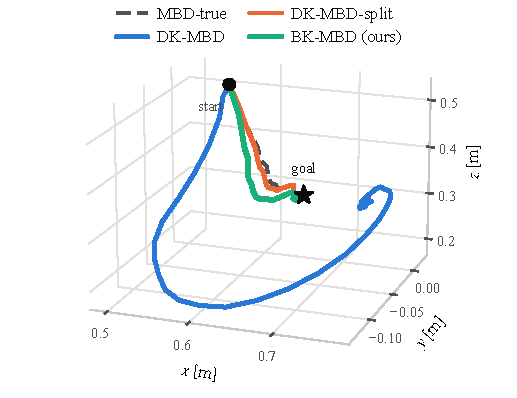
\includegraphics[width=\linewidth]{figs/traj_compare_adaptive.pdf}
\caption{Executed tool paths on one goal, one of the trials Table~\ref{tab:class} counts. The four runs share the planner, the training seed and the random stream, so they differ in the rollout model alone.}
\label{fig:paths}
\end{figure}

Two further conditions exclude the remaining explanations.
Raising the linear lift from $r = 20$ to $r = 50$ gave the linear model more parameters and more rollout arithmetic than the bilinear model, and it still reached $1/50$ and stopped a median $0.239$\,m away.
The bound \eqref{eq:bound} contains no lifted dimension, so a larger dictionary leaves the input sensitivity a single matrix.
The unstructured network reached $41/50$ within $5$\,cm and $0/50$ within $1$\,cm, stopping a median $0.054$\,m away.
Its input sensitivity depends on the state, so it can represent the input channel, and it did not identify that channel from the same data under the same objective.
Capacity and expressiveness therefore leave the failure in place, and the input channel accounts for it.

Table~\ref{tab:latency} reports the planning time per control step.
The oracle stepped the simulator at a median of $2598$\,ms and overran the $50$\,ms period at every one of its $1200$ control steps.
The bilinear rollout ran at a median of $11.0$\,ms with a worst case of $14.7$\,ms and missed no deadline over all $50$ trials.
The oracle is batched over four times the threads of the learned rollouts, so the count of Sec.~\ref{subsec:mbd} accounts for the gap.
One control step asks the rollout model for $NST = 60{,}000$ steps, which the $2$\,ms integrator turns into $1.5$ million physics substeps, and the $ST = 75$ batched steps among them lie on a serial chain.
The five stages run in series, so the period admits each of them within a $10$\,ms share.

\begin{table}[t]
\centering
\begin{threeparttable}
\caption{Planning time per control step over all trials.}
\label{tab:latency}
\footnotesize
\begin{tabularx}{\linewidth}{l Y Y Y}
\toprule
Rollout model & Median [ms] & Worst [ms] & Misses \\
\midrule
\mbdtrue{} & $2598$ & $2745$ & $1200$ \\
\dkmbd{} & $7.6$ & $12.5$ & $0$ \\
\bkmbd{} (ours) & $11.0$ & $14.7$ & $\mathbf{0}$ \\
\bottomrule
\end{tabularx}
\begin{tablenotes}[flushleft]\scriptsize
\item Misses counts control steps whose planning exceeded the $50$\,ms period.
\end{tablenotes}
\end{threeparttable}
\end{table}

The bilinear rollout cost $11.0$\,ms against $7.6$\,ms for the linear one, so the configuration-dependent input map is paid for well below the $m+1$ products a bilinear step issues, which share the lifted state they multiply.

\subsection{The Contribution of the Annealed Schedule}\label{subsec:exp_anneal}

This study holds the rollout class at the bilinear model and takes the noise schedule as the free variable.
Five schedules are compared at one total budget of $NS$ candidates per control step and at the temperature of Table~\ref{tab:hyper}, a single wide stage, a single narrow stage, $S$ wide stages, $S$ narrow stages, and the annealed schedule from wide to narrow.
The wide and narrow levels are the endpoints of the schedule in Table~\ref{tab:hyper}, $\sigma = 1.2$ and $\sigma = 0.3$.
The single-stage conditions draw $NS$ candidates at once, which by the third property of Sec.~\ref{subsec:mbd} is the MPPI update at the same budget and raises the sample count $S$-fold within one stage.
The tolerance is set to $1$\,cm, where the schedules separate, and they run on identical seeds, goals and planner streams, so every comparison below is paired.
The reaching task places no obstacle between the start and the goal, so its true cost admits a single basin, which is the condition Sec.~\ref{subsec:anneal} attaches to its prediction.

\begin{table}[t]
\centering
\begin{threeparttable}
\caption{Schedules at an equal total sample budget, tolerance $1$\,cm. The lower block repeats two of them on a rollout that carries no model error.}
\label{tab:anneal}
\footnotesize
\begin{tabularx}{\linewidth}{l Y Y}
\toprule
Schedule & Reach $1$\,cm & Final\tnote{a} \\
\midrule
\multicolumn{3}{@{}l}{\emph{Learned bilinear rollout}} \\
$1 \times NS$ wide (MPPI)\tnote{b} & $33/50$ & $0.010$ \\
$1 \times NS$ narrow (MPPI)\tnote{b} & $15/50$ & $0.041$ \\
$S \times N$ wide & $46/50$ & $0.012$ \\
$S \times N$ narrow & $26/50$ & $0.045$ \\
$S \times N$ anneal (ours) & $\mathbf{50/50}$ & $\mathbf{0.0097}$ \\
\midrule
\multicolumn{3}{@{}l}{\emph{True-dynamics rollout}\tnote{c}} \\
$S \times N$ narrow & $10/10$ & $0.009$ \\
$S \times N$ anneal & $10/10$ & $0.007$ \\
\bottomrule
\end{tabularx}
\begin{tablenotes}[flushleft]\scriptsize
\item[a] Median tracking error [m] at the end of the budget, which unlike the counts is not bounded by the tolerance.
\item[b] A single stage at a fixed noise level with $\eta = 1$ and no Langevin noise is the MPPI update at the same total sample budget.
\item[c] The oracle carries no learned model, so it is run over the $10$ goals alone, on the planner stream of the block above.
\end{tablenotes}
\end{threeparttable}
\end{table}

Table~\ref{tab:anneal} reports the outcome.
The annealed schedule reached the $1$\,cm band on all $50$ trials and left the lowest tracking error at the end of the budget.
Because the schedules run on the same goals, each comparison reads as a count of goals won and lost.
Against the two single-stage conditions the annealed schedule gains $17$ and $35$ goals and loses none, and against the staged wide and staged narrow schedules it gains $4$ and $24$.
Raising the sample count fivefold within one stage therefore does not substitute for the schedule, consistent with the logarithmic dependence in \eqref{eq:reach}.

Rolling the settled plan of each schedule through the model and through the true dynamics locates where each one stops.
Under the narrow schedule the model puts the terminal error of that plan at $0.024$\,m while the plant delivers $0.053$\,m, so the schedule has settled on a minimum of the surrogate.
The annealed schedule returns $0.020$\,m against a plant value of $0.015$\,m and settles where the two landscapes agree.

We then repeated two schedules on the true-dynamics rollout, over the same goals and the same planner stream.
The schedules stop separating.
The narrow schedule reaches the $1$\,cm band on $10/10$ goals as the annealed schedule does, against $26/50$ under the learned rollout (Fisher exact, $p = 0.003$), and its settled error moves from $0.045$ to $0.009$\,m.
The narrow level settles quickly on either rollout, so what it loses under the learned one is the surrogate rather than the sampling.

The wide level pays at the other end.
Table~\ref{tab:step} reports the control displacement one control step produces and the tracking error it removes.
The displacement grows by a factor of $3.8$ from $\sigma = 0.3$ to $\sigma = 1.2$ while the error removed falls, so the error removed per unit of control drops by a factor of six.
The efficiency falls monotonically with the noise level, which is what \eqref{eq:step} and the smoothing of Sec.~\ref{subsec:anneal} lead one to expect.
The wide schedules therefore come to rest within a centimetre of the goal and still miss the band.
No fixed level therefore meets both conditions at once.
The annealed schedule executes at the displacement of the narrow level, $0.109$, retains an efficiency of $48.4$ against the $9.9$ of the wide level, and reaches on all $50$ goals.
Its displacement coincides with the narrow level because the wide stages select the basin while the last stage produces the executed step.

\begin{table}[t]
\centering
\begin{threeparttable}
\caption{Step size and step quality at a fixed noise level.}
\label{tab:step}
\footnotesize
\begin{tabularx}{\linewidth}{l Y Y Y}
\toprule
$\sigma$ & $|\Delta U|$ & Error removed & Efficiency\tnote{a} \\
\midrule
$0.3$ & $0.109$ & $0.00665$ & $61.7$ \\
$0.8$ & $0.292$ & $0.00571$ & $19.2$ \\
$1.2$ & $0.418$ & $0.00409$ & $9.9$ \\
anneal & $0.109$ & $0.00525$ & $48.4$ \\
\bottomrule
\end{tabularx}
\begin{tablenotes}[flushleft]\scriptsize
\item[a] Error removed per unit of control displacement, scaled by $10^{3}$. $|\Delta U|$ is the displacement of the plan over one control step and the error removed is the reduction in tracking error over that step, both averaged over control steps and trials.
\end{tablenotes}
\end{threeparttable}
\end{table}

\subsection{Non-Convex Passage}\label{subsec:exp_window}

This study holds the rollout model fixed and exchanges the optimizer.
A wall carries a single circular aperture, the start lies on the near side, and the goals are sampled on the far side.
The straight chord from the start to any goal crosses the wall below the aperture, so every reaching motion must route through the opening (Fig.~\ref{fig:window}).
The drone flies this task over $50$ trials, and at each trial the two planners receive one trained bilinear model.
\bkmbd{} absorbs the wall into the cost as a penalty, which Sec.~\ref{subsec:problem} leaves to the optimizer.
The convexified controller instead relinearizes the keep-out set at every step and solves the resulting quadratic program over four sequential iterations along the nominal bilinear rollout~\cite{bruder2021bilinear}.

\begin{figure}[t]
\centering
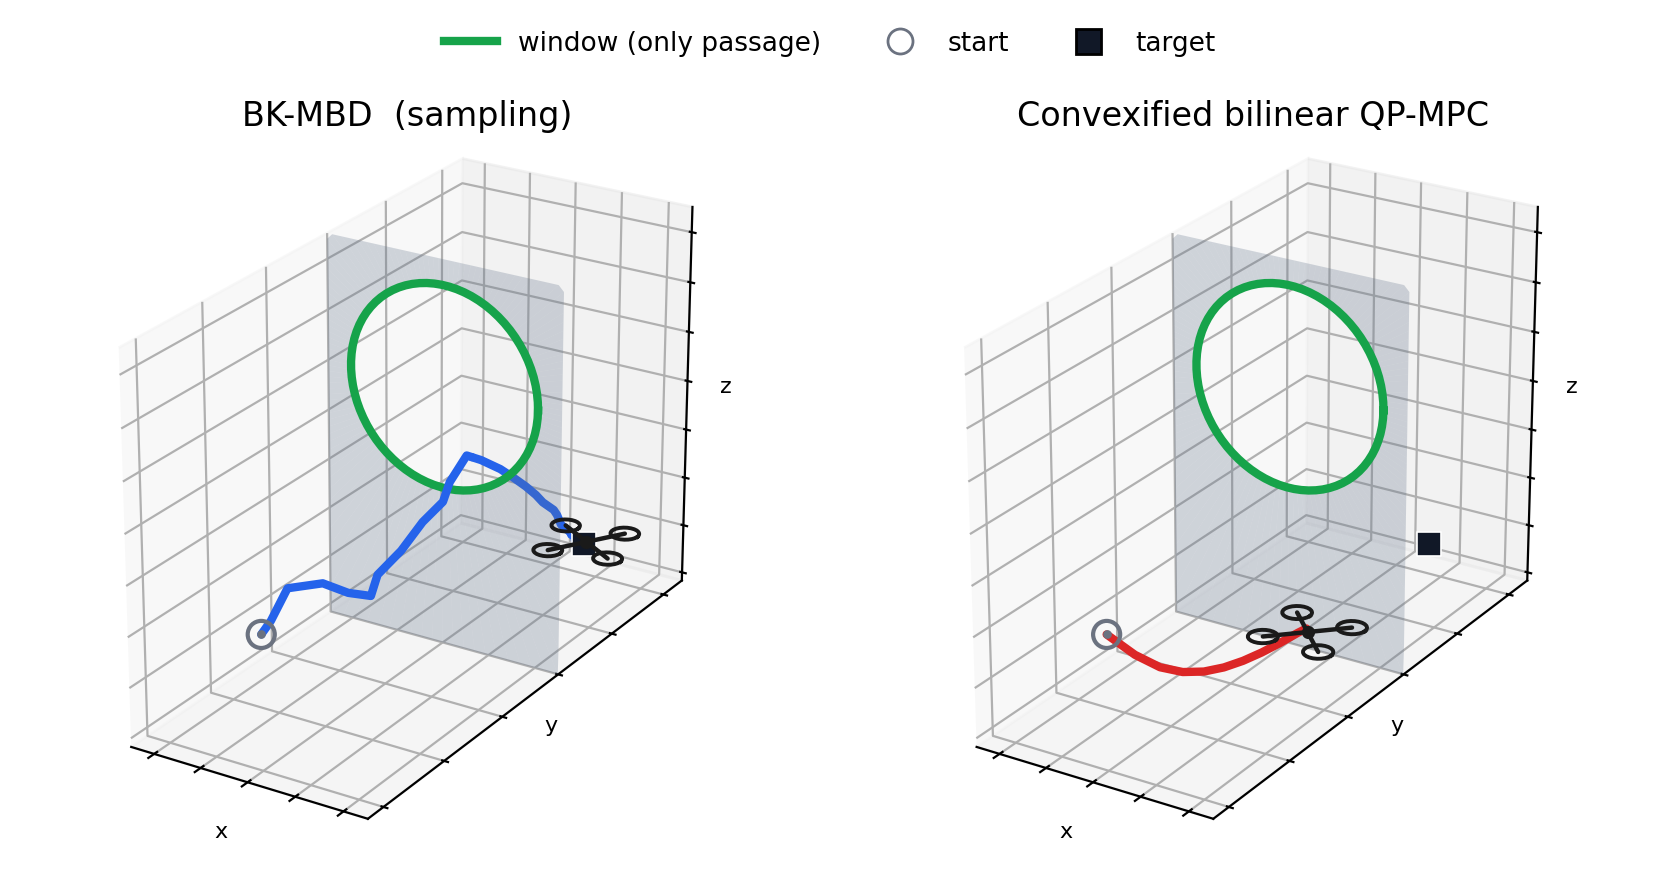
\includegraphics[width=\linewidth]{figs/drone_window.png}
\caption{Non-convex passage on the drone. The wall admits a single circular aperture. \bkmbd{} (left) threads the aperture and reaches the far-side goal, while the convexified bilinear controller (right) holds the near side.}
\label{fig:window}
\end{figure}

\bkmbd{} reached the $1$\,cm tolerance on $50/50$ goals and the convexified controller on $10/50$, and both executed zero constraint violations.
Every failure of either planner was a stall at a collision-free pose, so on identical goals the two separated on passage completion at equal safety.

The structure of the free space accounts for the convexified controller.
That space is the union of the two sides of the wall joined through the aperture, and a convex program retains one region containing the current nominal.
Any such region that excludes the wall lies entirely on the near side.
The far-side goal therefore falls outside the feasible set at every step, and the solve converges to the point of its own region closest to the goal.
Two measurements match that account.
The convexified controller settled a median of $0.030$\,m from the wall, which is the planning margin of its own keep-out set.
The ten goals it did reach were the ten whose offset from the aperture axis was smallest, at most $0.148$\,m against a median of $0.291$\,m over all goals.
\bkmbd{} scores whole candidate sequences by the cost they achieve, so a candidate routed through the aperture receives its weight from the outcome it produces.

Two convexifications act on that controller at once, one of the dynamics and one of the free space.
The two measurements above bear on the second.
A controller limited by the frozen dynamics would fail by tracking a poor nominal, whereas this one stalls at the margin of its own keep-out set and succeeds on exactly the goals nearest the aperture axis.
We therefore attribute the separation to the convexification of the free space, and remedies that partition that space into several convex regions remain open.

\todo{Hardware study (\texttt{subsec:exp\_hw}) to follow.}

%==============================================================
\section{Conclusion}\label{sec:conclusion}
%==============================================================

\todo{To be written last.}

\bibliographystyle{IEEEtran}
\bibliography{IEEEabrv,ours}

\end{document}